\chapter{Evaluating dark matter signals}

The main goal of the thesis is to investigate if certain dark matter signals can be detected after the high luminosity upgrade. One immediate worry is that the background will be large in comparison to the signal, making the signal undetectable.

Another goal is to investigate if it might become more difficult to differentiate between the signal and background due to the degradation of jet and missing energy resolutions in the high luminosity upgrade.

This thesis focus on using a luminosity at 1000 fb$^{-1}$ and a center of mass energy at 14 TeV. The reco data is created using a pile-up rate, $\obs{\mu} = 140$ as expected during phase II.

The signal models are given in \appendixref{cha:datasets} along with the background models. The different models were introduced \subsectionref{sec:tb:subsec:eft} and will be discussed in more detail in this chapter.

Each signal model has been evaluated in different signal regions and the detectability has been evaluated using a statistical P-value. This process has been performed at a pile-up value of 140, as expected for after the high luminosity upgrade. 

\newpage
\section{Signal to background ratio}
\subsection{Signal Region}
A signal region (\abbrSR) is defined as a set of selections on event variables designed to create a sample which is enriched in signal and depleted of background. One usually tries to design the signal region so that the signal is large enough and the background small enough that one would statistically be able to either:
\begin{itemize}
\item Exclude the signal if the observation of the data is compatible with a background only hypothesis.
\item Detect the signal and quantify the significance of the excess in data over background if the data is consistent with a signal + background hypothesis.
\end{itemize}

An event is a recorded proton-proton collision which consists of hundreds or thousands of observables such as the number of electrons, muons, jets, tau leptons, gammas or E$^{Miss}_T$ each with their energy and momenta.

To define an optimal signal region is not known a priori and has to be studied for different signal models. The optimal region typically changes e.g with a change of the mass of new particles for instance the \abbrWIMP mass or the suppression scale. This is why there are several different signal regions to be studied in this thesis.

\subsection{Weight}
A weight is used to normalize different types of data so that they can be compared. 
As given in \eqref{eq:Numevents}, the total number of events can be estimated as:
\begin{equation}
N=\sigma \int \mathscr{L} dt \equiv \sigma \Lagr
\end{equation}
Thus, if all events are generated at different luminosities, depending on the computing power of the computer which performed the simulation, the following weight should be used to receive the events at a new luminosity:
\begin{equation}
weight=\frac{\Lagr \sigma}{N_{Raw}}
\end{equation}
where $N_{Raw}$ is the number of events expected at the luminosity that was set to create the data, compared to $\Lagr$ which is the luminosity at which the data is compared and $\sigma$ is the cross-section. In this thesis the luminosity is fixed at $\Lagr=1000$fb$^{-1}$.

\subsection{Verification of background normalization} 	
To verify that the background samples are correctly normalized they are compared with Ref. \citep{ATLAS-CONF-2012-147} in which the center of mass energy is 8 TeV and the luminosity is 10 fb$^{-1}$. Since the luminosity is not 1000 fb$^{-1}$ as used in this thesis the expected values from the paper scaled up with a factor 100 to be comparable. 

Somewhat unexpectedly a center of mass energy at 8 TeV had cross-sections a factor 4 lower than the cross-sections at 14 TeV. 
These cross-sections are generated either with MadGraph\citep{madgraph} or PYTHIA\citep{Sjostrand:2008} depending on the generator given for each dataset in \appendixref{cha:datasets}. 

The signal regions used in the article were the following:
\begin{table}[h]
\begin{center}
\begin{tabular}{l}
\hline
Selection Criteria \\ \hline
Jet veto, require no more than 2 jets with $p_T > 30 GeV$ and $|\eta| < 4.5$ \\
Lepton veto, no electron or muon \\
Leading jet with $|\eta| < 2.0$ and $\Delta \phi (jet, E_T^{Miss})>0.5$ (second-leading jet) \\ \hline
\end{tabular}
\begin{tabular}{l l l l l l}
signal region & SR3p & SR4p \\ \hline
minimum leading jet p$_T$ (GeV) & 350 & 500 \\
minimum E$^{Miss}_T$ (GeV) & 350 & 500 \\ \hline
\end{tabular}
\label{tab:oldsr}
\caption{The signal regions from Ref. \citep{ATLAS-CONF-2012-147}.}
\end{center}
\end{table}

The article \citep{ATLAS-CONF-2012-147} has in total four signal regions, unfortunately since the simulated events used in this thesis are filtered before the analysis only the two highest regions are comparable. This can be seen in \tableref{tab:Compare1} in \subsectionref{Verifying background data}.

\subsection{Errors in data}\label{subsec:errdata}
To make a through analysis of the background it is important to take into consideration different errors that exist in the number of events. This is especially important when looking at which signals can be excluded in different signal regions.
There exists three main types of errors:
\begin{itemize}
\item Statistical errors from \abbrMC.
\item Statistical errors from the control region. 
\item Systematic errors.
\end{itemize}
The statistical errors from \abbrMC come from the method of generating background events and is unfortunately nothing that can be estimated when one is not generating the events. 

The statistical errors from the control region require an explanation of what a control region is. A control region (\abbrCR) is similar to a signal region, a set of criteria which are imposed on the data. This criteria are set so that there can be a region with almost no signal. In this \abbrCR there will still be fluctuations in the amount of background events due to statistical effects, which can then be measured. 

The systematic errors is a fixed error which is always present coming from different approximations in how all the events were generated. 

\subsection{Figure of merit}\label{subsec:figmer}
To be able to evaluate different signal regions and different signal models, a figure of merit p is used. The value p is the probability for the background to fluctuate to the value of the signal + background. Thus if the p-value is small, regardless if the signal is large or the background or its fluctuations are small, it is improbable that the background could result in the same value as if there was a signal and background. This means that for a sufficiently small p-value the signal is detectable.  

Assuming the expected number of background events are B $\pm \sigma_B$ where $\sigma_B$ is the quadratic sum of the statistical error from Monte Carlo, the statistical error from the control region (\abbrCR) and the systematic errors as explained in \subsectionref{subsec:figmer}. The expected number of signal events is S, assumed without fluctuation. 

If no uncertainty in B or S is assumed, then the probability that the background will fluctuate up to the signal and background should follow a Poisson distribution as such:
\begin{equation}
\text{P(S+B|B)}=\frac{e^{-B}B^{(S+B)}}{(S+B)!}
\end{equation} 

The probability that the background will fluctuate to a value N larger or equal to the signal and background then becomes:
\begin{equation}
\text{P(B$ \geq$S+B|B)} \equiv \text{P(N|B)}=\sum_{N=S+B}^{\infty}  \frac{e^{-B}B^N}{N!}
\end{equation} 

However since there is an uncertainty in the background, the probability distribution P(N|B) must be convoluted with a Gaussian function:
\begin{equation}
 \text{G(N$_B$|B,$\sigma_B$)}=\frac{1}{\sigma_B \sqrt{2 \pi}} e^{-\frac{(N_B-B)^2}{2\sigma_B^2}}
\end{equation}
where N$_B$ is the expected number of background events. The convolution is done using N$_B$ as B resulting in the total probability density function:
\begin{align}
\text{F(N|N$_B$},\sigma_B) &= \text{P(N|B)$\ast$G(N$_B$|B,$\sigma_B$)}= \notag \\
&=\int\limits_{-\infty}^{\infty}P(N|N_B - B)G(N_B|B,\sigma_B) dN_B
\end{align}
Inserting the sum over N leads to the probability of the background fluctuation to signal and background being obtained as.
\begin{equation}
p = \sum\limits_{N=S+B}^{\infty} \int\limits_{-\infty}^{\infty} \text{P(N|N$_B - $B)G(N$_B$|B,$\sigma_B$)} dN_B
\end{equation}

In this thesis, two different models of the error in the background $\sigma_B$ are used.   
Both models are based on Ref. \citep{ATLAS-CONF-2012-147}. As described in the beginning of this subsection the error is calculated as:
\begin{equation*}
\sigma_B = \text{Statistical error from \abbrMC} \oplus \text{Statistical error in \abbrCR} \oplus \text{Systematic error}
\end{equation*}

\begin{itemize}
\item The statistical error from \abbrMC has been neglected since there is no way of estimating it.
\item The statistical error from background \abbrCR has been take from the article and assumed to decrease with the increased luminosity as, $\frac{30}{380} \frac{\sqrt{L_{old}}}{\sqrt{L_{new}}}$
\item The systematic error has been given two different values, from the article:\\ $\frac{30}{380}$ or fixed at 0.02.
\item All this results the total error being used as either, 0.08 or 0.02. 
\end{itemize}

\subsection{D5 operator models}\label{sec:signal:subsec:d5}
As described in \subsectionref{sec:tb:subsec:eft}, one of the signals is modelled using the D5 operator. In this thesis two different scenarios are used, one at a dark matter mass of 50 GeV and one at 400 GeV.

Each of these models are modelled with a mass suppression scale, denoted M*, which is connected to the cross-section of the process through:
\begin{equation}
\sigma_{new} = \frac{\sigma_{old}}{M^*} 
\end{equation}

In \subsectionref{sec:res:subsec:m*} it is determined which values of M* could be excluded with the upgraded \abbrLHC phase 2 upgrade and \abbrATLAS .

\subsection{Light vector mediator models}\label{sec:signal:subsec:vecmed}
As described in \subsectionref{sec:tb:subsec:eft}, the other signal model is a vector mediator model. In this thesis these signals have two different width scenarios and a number of different mediator mass scenarios. \textbf{Where width is related to the lifetime of the dark matter particle.} In addition to this there are, as with the D5 operator, two different dark matter masses, one at 50 GeV and one at 400 GeV.

The result of the investigation of which models are excludable with the upgraded \abbrLHC phase 2 upgrade and \abbrATLAS are given in \subsectionref{sec:res:subsec:Mm}. 
 
\newpage
\section{Signal region definitions}
\subsection{Signal regions}
To be able to compare signal results to previous papers new signal regions were devised. It was also discovered that the requirement of no electrons or muons was to harsh for the signal models. Because of this new signal criteria were devised.

\begin{table}[h]
\begin{center}
\begin{tabular}{l}
\hline
Selection Criteria \\ \hline
Jet veto, require no more than 2 jets with $p_T > 30 GeV$ and $|\eta| < 4.5$ \\
Lepton veto, no electron or muon. \\
The electron veto is defined: $\Delta R (jet^{lead},electron^{lead})\geq 0.4$ and \\
$electron^{lead} P_T>20 GeV$ removed.\\
The muon veto is defined: $\Delta R (jet^{lead},muon^{lead})\geq 0.4$ and \\
$muon^{lead} P_T>20 GeV$ removed.\\
Leading jet with $|\eta| < 2.0$ and $\Delta \phi (jet, E_T^{Miss})>0.5$ (second-leading jet) \\ 
\end{tabular}
\begin{tabular}{l l l l l l}
\hline
signal region & SR1 & SR1p & SR2 & SR3 & SR4 \\ \hline
minimum leading jet p$_T$ (GeV) & 350 &500& 600 & 800 & 1000 \\
minimum E$^{Miss}_T$ (GeV) & 350&500 & 600 & 800 & 1000 \\
\end{tabular}
\begin{tabular}{l l l l l} \hline
signal region & SRa &  SRb & SRc & SRd \\ \hline
minimum leading jet p$_T$ (GeV) & 350 & 350 & 350 & 350 \\
minimum E$^{Miss}_T$ (GeV) & 350 & 600 & 800 & 1000 \\ \hline
\end{tabular}
\label{tab:newsr}
\caption{The new signal regions}
\end{center}
\end{table}

\subsection{Verifying background data}
To make sure that the altered electron veto still produces results comparable with \citep{ATLAS-CONF-2012-147} a comparison is made again. This can be seen in \subsectionref{Verifying background data} in \tableref{tab:newcomp}.

\section{Mitigating the effect of the high luminosity}
As discussed in \subsectionref{chap:vali:sec:dis:subsec:smearindep} the smearing functions effect of pile-up should be minimal in the high energy regions which are of interest in this thesis. 

From the formulation of the smearing functions, the biggest effect should be seen at low energies. This is related to the difficulty for the hardware triggers to select events. This means that one drawback of the high luminosity upgrade is that very low energy signal regions will be lost.

The effect of the high luminosity is seen in \chapterref{chap:sig:sec:res} and discussed in \subsectionref{subsec:hleff}.

\newpage
\section{Results}\label{chap:sig:sec:res}
\subsection{Verifying background data}\label{Verifying background data}
In \tableref{tab:Compare1} and  \tableref{tab:newcomp} a comparison has been made between the number of simulated background events at a truth level and the number of expected events by scaling up the values from Ref. \citep{ATLAS-CONF-2012-147} by a factor 100. Truth data was used to not let the increased pile-up value affect the comparison. It can be seen that the simulated events and expected events coincide quite well on all accounts apart from W$\rightarrow\tau\nu$, W$\rightarrow\mu\nu$ and thus the total as well. 

The difference in W$\rightarrow\tau\nu$ can be explained by the fact that $\tau$ can not be recreated as a jet in the simulated events which it can in measured events.

The difference in W$\rightarrow\mu\nu$ is explained through the simulated events having a better separation of muons neutrinos and E$_T^{Miss}$.

\begin{table}[ht]
\begin{center}
\begin{tabular}{|l|l|l|l|l|}
\hline
& \multicolumn{2}{c}{SR3p} & \multicolumn{2}{|c|}{SR4p} \\
\hline
Process & Simulated & From paper & Simulated & From paper \\ \hline
Z$\rightarrow\nu\nu$ & 140298 & 152000 & 25250 & 27000 \\
W$\rightarrow\tau\nu$ & 40701 & 37000 & 5862 & 3900 \\
W$\rightarrow e\nu$ & 11229 & 11200 & 1507 & 1600 \\
W$\rightarrow\mu\nu$ & 13727 & 15800 & 1872 & 4200 \\ \hline
Total background & 205955 & 218000 & 34491 & 36700 \\ \hline
\end{tabular}
\caption{Comparison of the simulated and expected events from Ref. \citep{ATLAS-CONF-2012-147} with $\Lagr=1000$fb$^{-1}$, cross-sections corresponding to $\sqrt{s}=8$TeV and using the same electron and muon veto.}
\label{tab:Compare1}
\end{center}
\end{table}

\begin{table}[ht]
\begin{center}
\begin{tabular}{|l|l|l|l|l|}
\hline
& \multicolumn{2}{c}{SR1} & \multicolumn{2}{|c|}{SR1p} \\
\hline
Process & Simulated  & From paper & Simulated & From paper  \\ \hline
Z$\rightarrow\nu\nu$ & 150753 & 152000 & 27569 & 27000 \\
W$\rightarrow\tau\nu$ & 49320 & 37000 & 7318 & 3900 \\
W$\rightarrow e\nu$ & 18329 & 11200 & 2534 & 1600 \\
W$\rightarrow\mu\nu$ & 22290 & 15800 & 3218 & 4200 \\ \hline
Total background & 240690 & 218000 & 40639 & 36700 \\ \hline
\end{tabular}
\caption{Comparison of the simulated and expected events from Ref. \citep{ATLAS-CONF-2012-147} with $\Lagr=1000$fb$^{-1}$, cross-sections corresponding to $\sqrt{s}=8$TeV and using a modified electron and muon veto.}
\label{tab:newcomp}
\end{center}
\end{table}


\subsection{Events}
In the following tables the number of events are given using one of the D5 operators as the signal, and the background in the different signal regions. The number of background events is also used for the vector mediator signals.

%\renewcommand{\arraystretch}{1.0} %Change back
%\renewcommand{\arraystretch}{1.5} %Change height of tabel
\begin{landscape}
\begin{table}[ht]
\begin{center}
\begin{tabular}{|l|l|l|l|l !{\vrule width 4pt} l|l|l|l|}
\hline
Process at $\sqrt{s}=14$TeV& SR1 & SR2 & SR3 & SR4 & SRa & Srb & Src & Srd \\ \hline
D5, mDm=50 GeV, M*=1TeV & 131844 & 30900 & 11053 & 4532 & 131844 & 37217 & 13280 & 5387 \\ \hline
Z$\rightarrow\nu\nu$ & 619752 & 44146 & 8764 & 2205 & 619752 & 61193 & 11975 & 2998 \\
W$\rightarrow\tau\nu$ & 169983 & 8753 & 1479 & 344 & 169983 & 12047 & 2032 & 453\\ 
W$\rightarrow e\nu$ & 63026 & 2986 & 510 & 114 & 63026 & 4114 & 688 & 160 \\
W$\rightarrow\mu\nu$ & 76618 & 3880 & 658 & 162 & 76618 & 5094 & 871 & 199 \\ \hline
Total background & 929379 & 59765 & 11411 & 2825 & 929379 & 82448 & 15566 & 3810 \\ \hline
\end{tabular}
\caption{Signal and background events for truth data in the signal regions.}
\label{tab:srtruth1}
\end{center}
\vspace*{5px}
\begin{center}
\begin{tabular}{|l|l|l|l|l !{\vrule width 4pt} l|l|l|l|}
\hline
Process at $\sqrt{s}=14$TeV& SR1 & SR2 & SR3 & SR4 & SRa & SRb & SRc & SRd \\ \hline
D5, mDm=50 Gev, M*=1TeV & 122117 & 28663 & 10273 & 4259 & 122117 & 39618 & 14151 & 5679 \\ \hline 
Z$\rightarrow\nu\nu$ & 568410 & 40518 & 8012 & 2023 & 568410 & 74564 & 13817 & 3318 \\
W$\rightarrow\tau\nu$ & 170999 & 8644 & 1442 & 314 & 170999 & 16241 & 2446 & 536 \\
W$\rightarrow e\nu$ & 60071 & 2799 & 470 & 110 & 60071 & 5366 & 835 & 183 \\
W$\rightarrow\mu\nu$ & 73495 & 3704 & 629 & 152 & 73495 & 6622 & 1046 & 236 \\ \hline
Total background & 872975 & 55665 & 10552 & 2599 & 872975 & 102793 & 18144 & 4273 \\ \hline 
\end{tabular}
\caption{Signal and background events for reco data with $\obs{\mu}=140$ in the signal regions.}
\label{tab:srreco1}
\end{center}
\end{table}

Note how the ratio between the number of signal events and total background increases from the first to the last signal regions meaning that these are good choices of signal regions. Also note how similar the two tables are even though \tableref{tab:srreco1} is at reco with a pile-up rate of 140.
\end{landscape}

\subsection{Limit on M*}\label{sec:res:subsec:m*}
For the D5 operators as described in \subsectionref{sec:signal:subsec:d5} limits on the mass suppression has been calculated by evaluating at which point the signal is covered by the background, meaning that the p-value $>0.05$. This is done using the two different error models as described in \subsectionref{subsec:figmer} as figures of merit.

The limit is found, seen as a horizontal line in both \figureref{fig:SRnewMt} and \figureref{fig:SRnewMr}, when the p-value = 0.05. In these images the effect of a change of error model can be seen as a left shift but no change in incline.

 \begin{figure}[H] %!ht
    \subfloat[ \label{fig:SRnewMt:1}]{%
     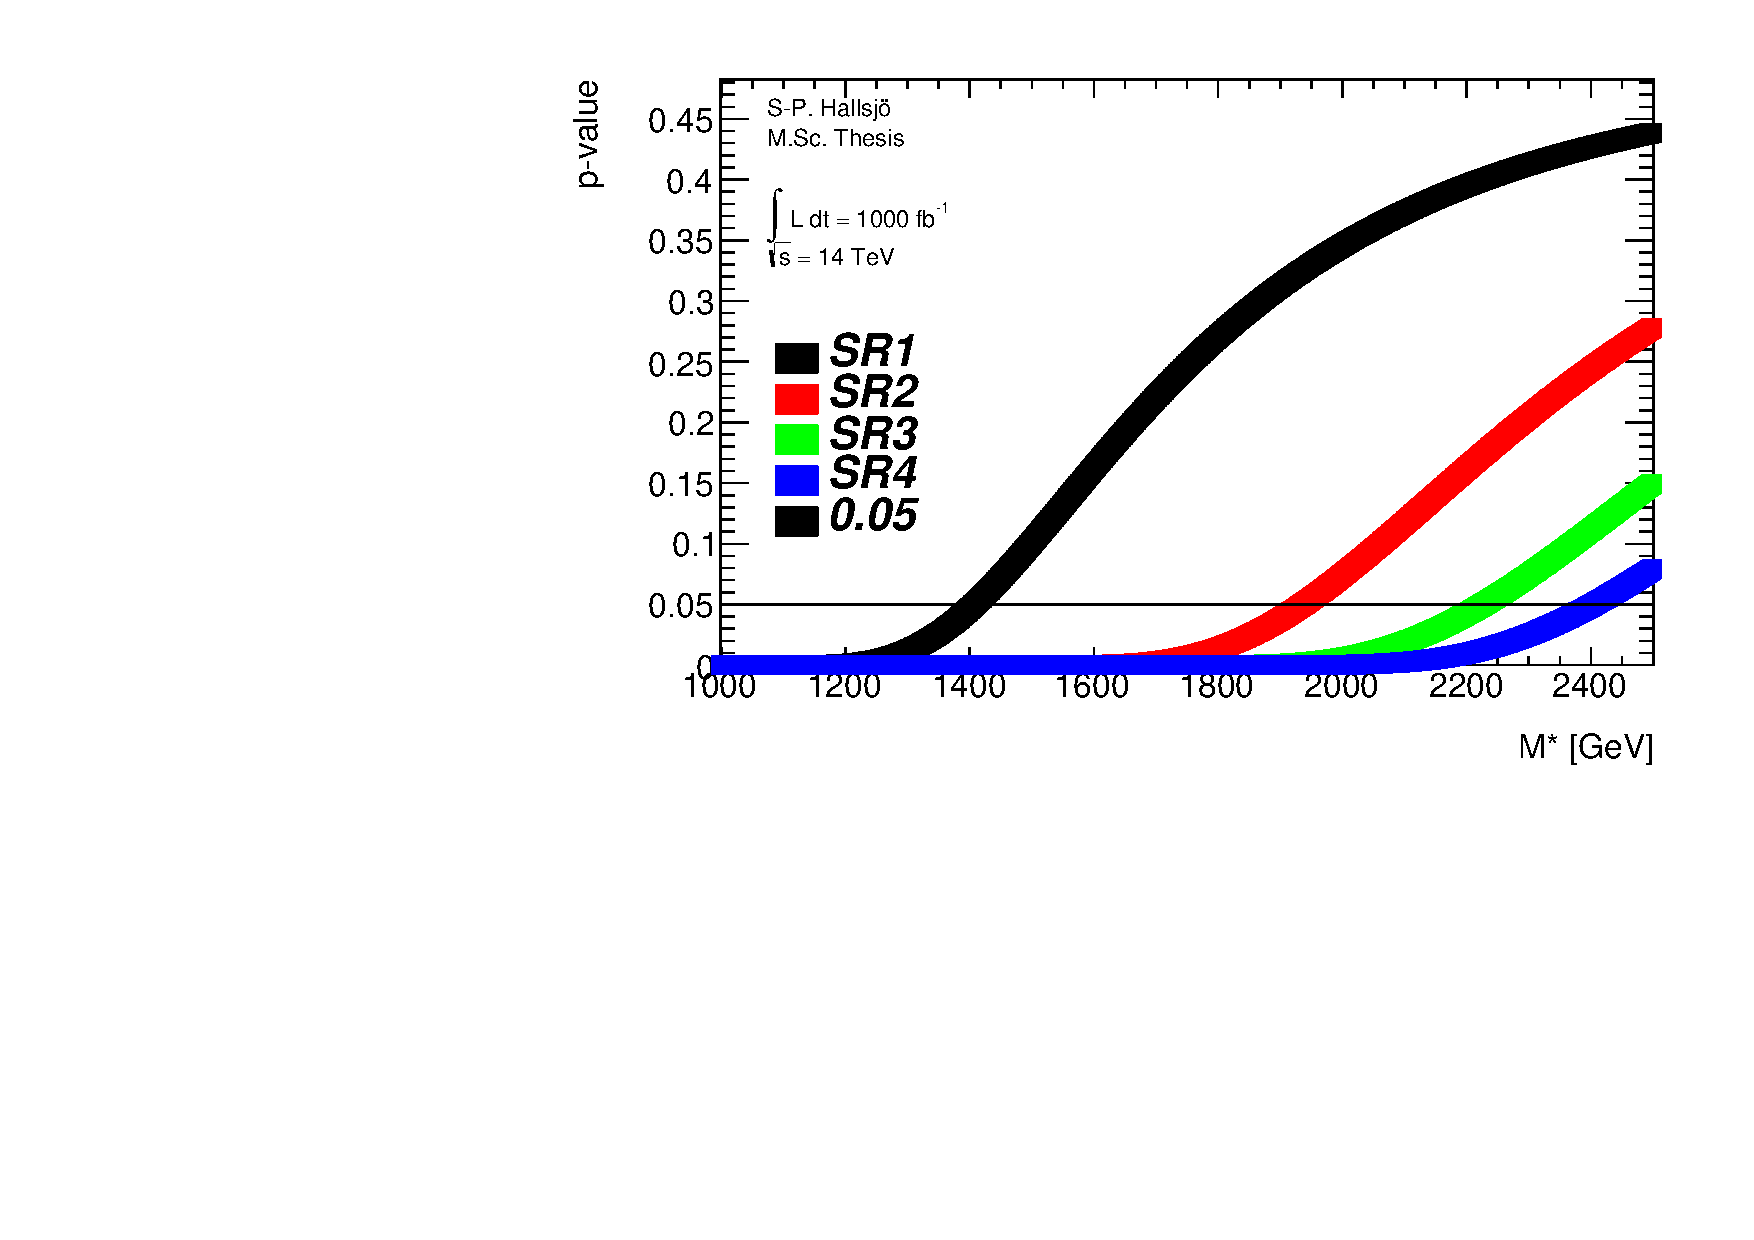
\includegraphics[width=0.5\textwidth]{pvald5002truth2.pdf}
    }
    \hfill
    \subfloat[ \label{fig:SRnewMt:2}]{%
      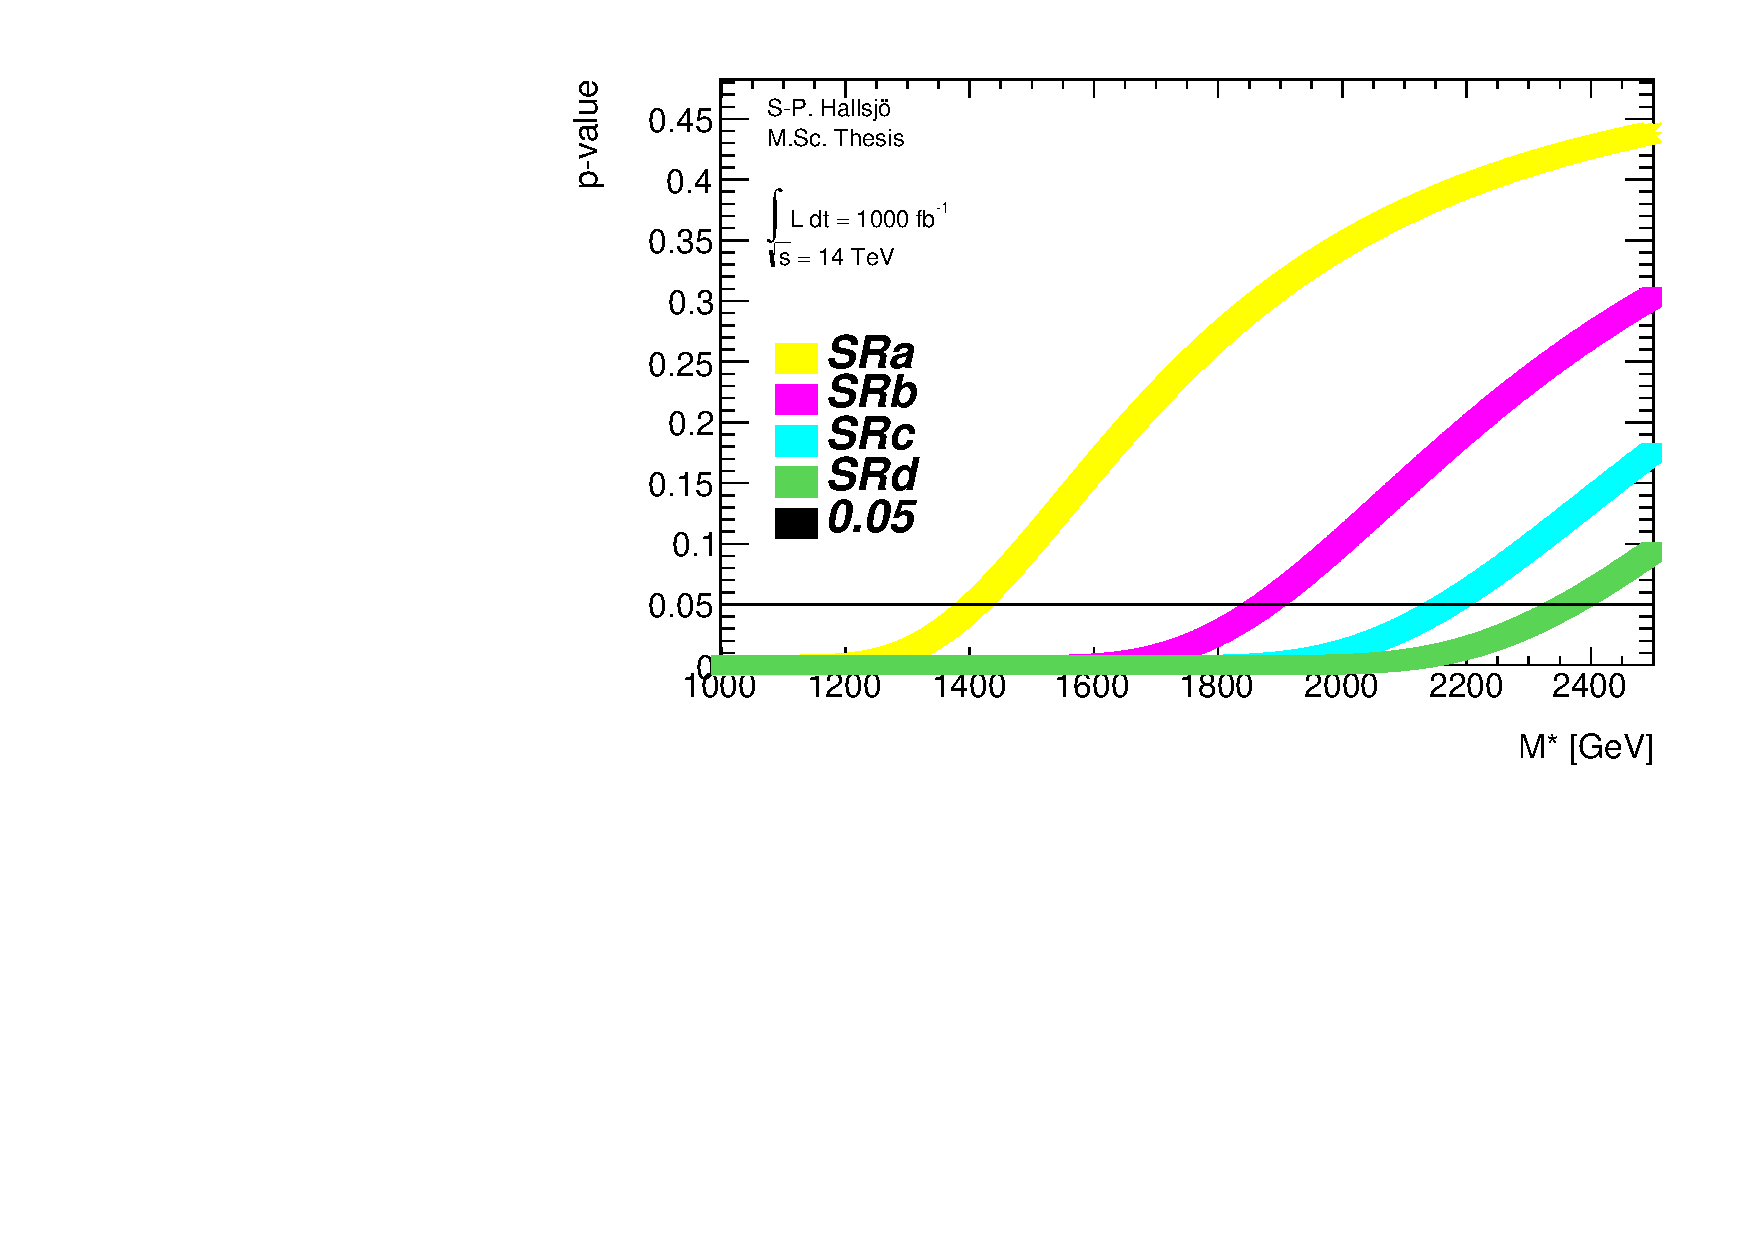
\includegraphics[width=0.5\textwidth]{pvald5002truth.pdf}
    }
    \caption{Limits of the mass suppression on a truth level for error model 0.02.}
    \label{fig:SRnewMt}
  \end{figure}

 \begin{figure}[H] %!ht
    \subfloat[ \label{fig:SRnewMr:1}]{%
     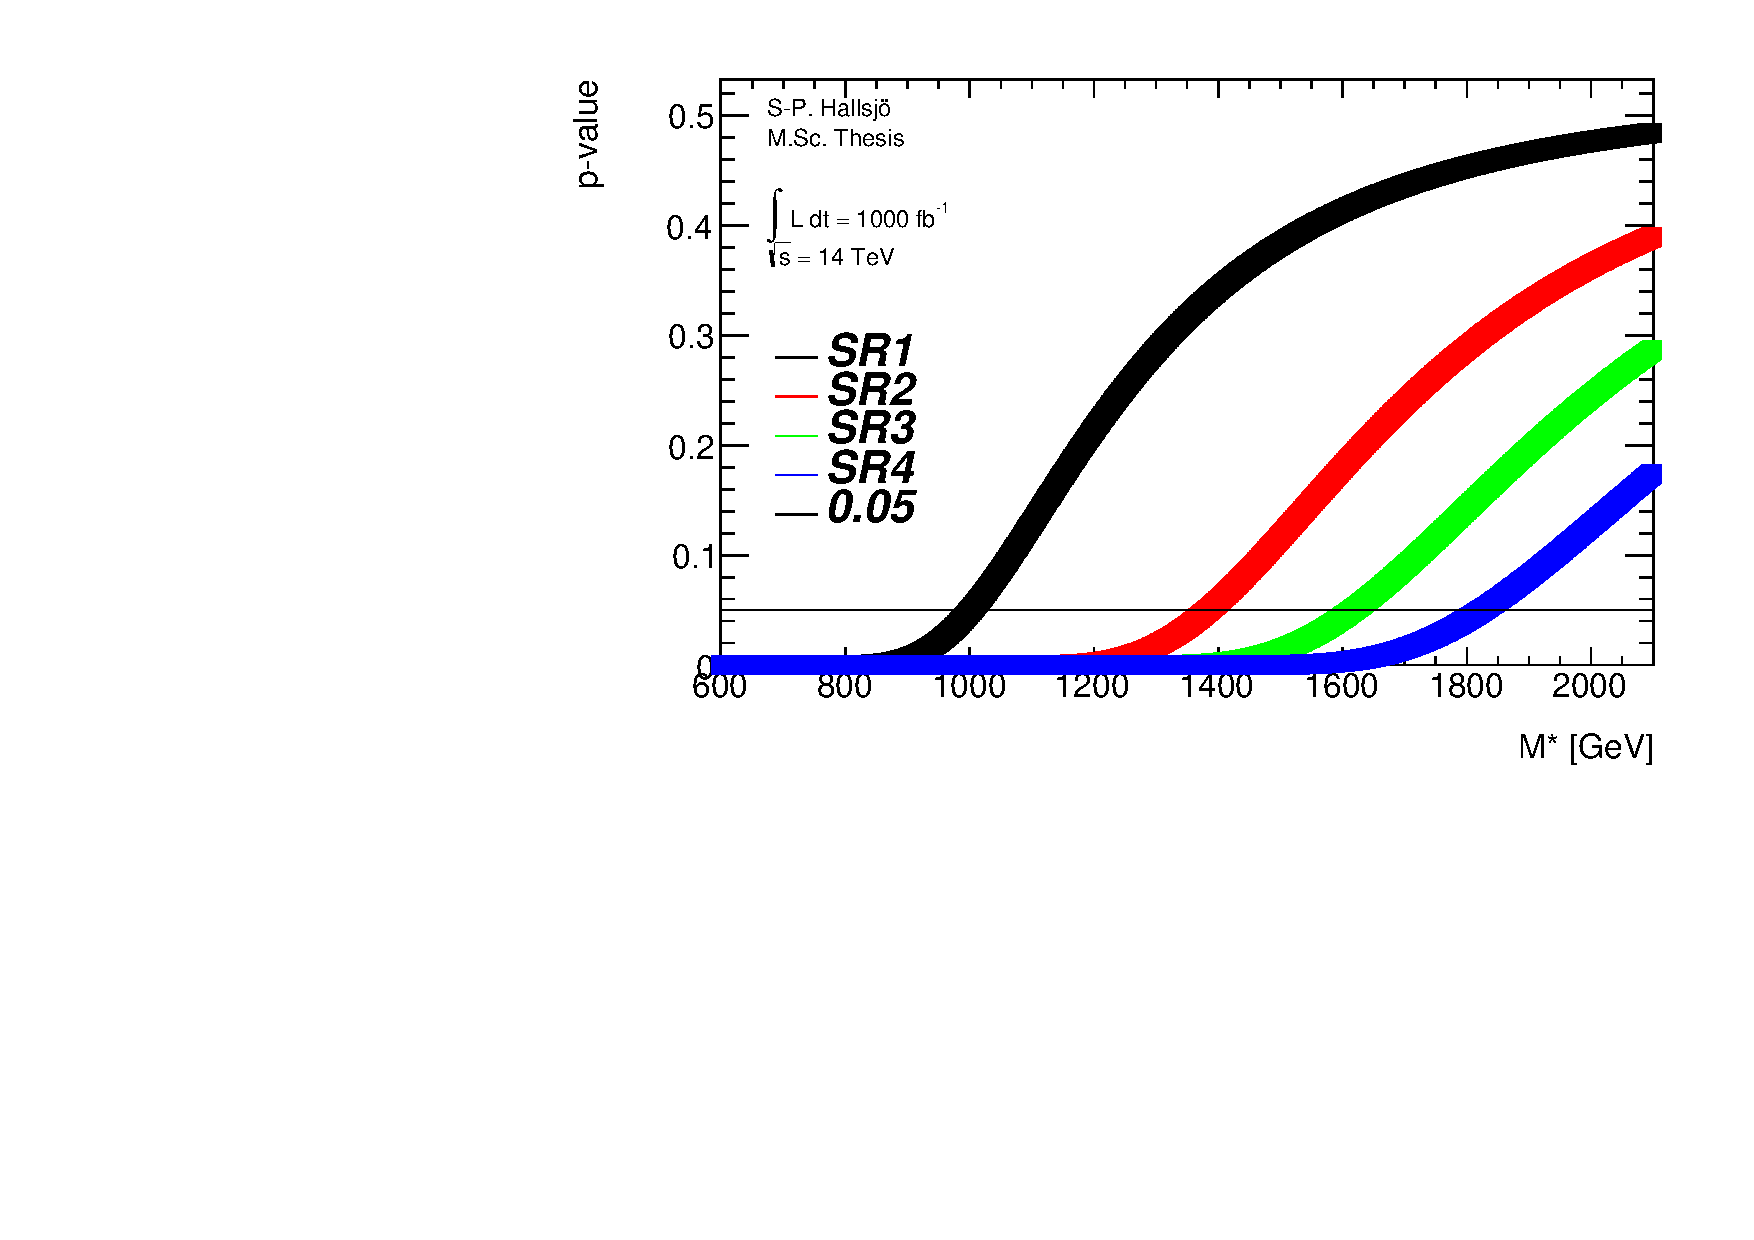
\includegraphics[width=0.5\textwidth]{pvald5008truth2.pdf}
    }
    \hfill
    \subfloat[ \label{fig:SRnewMr:2}]{%
      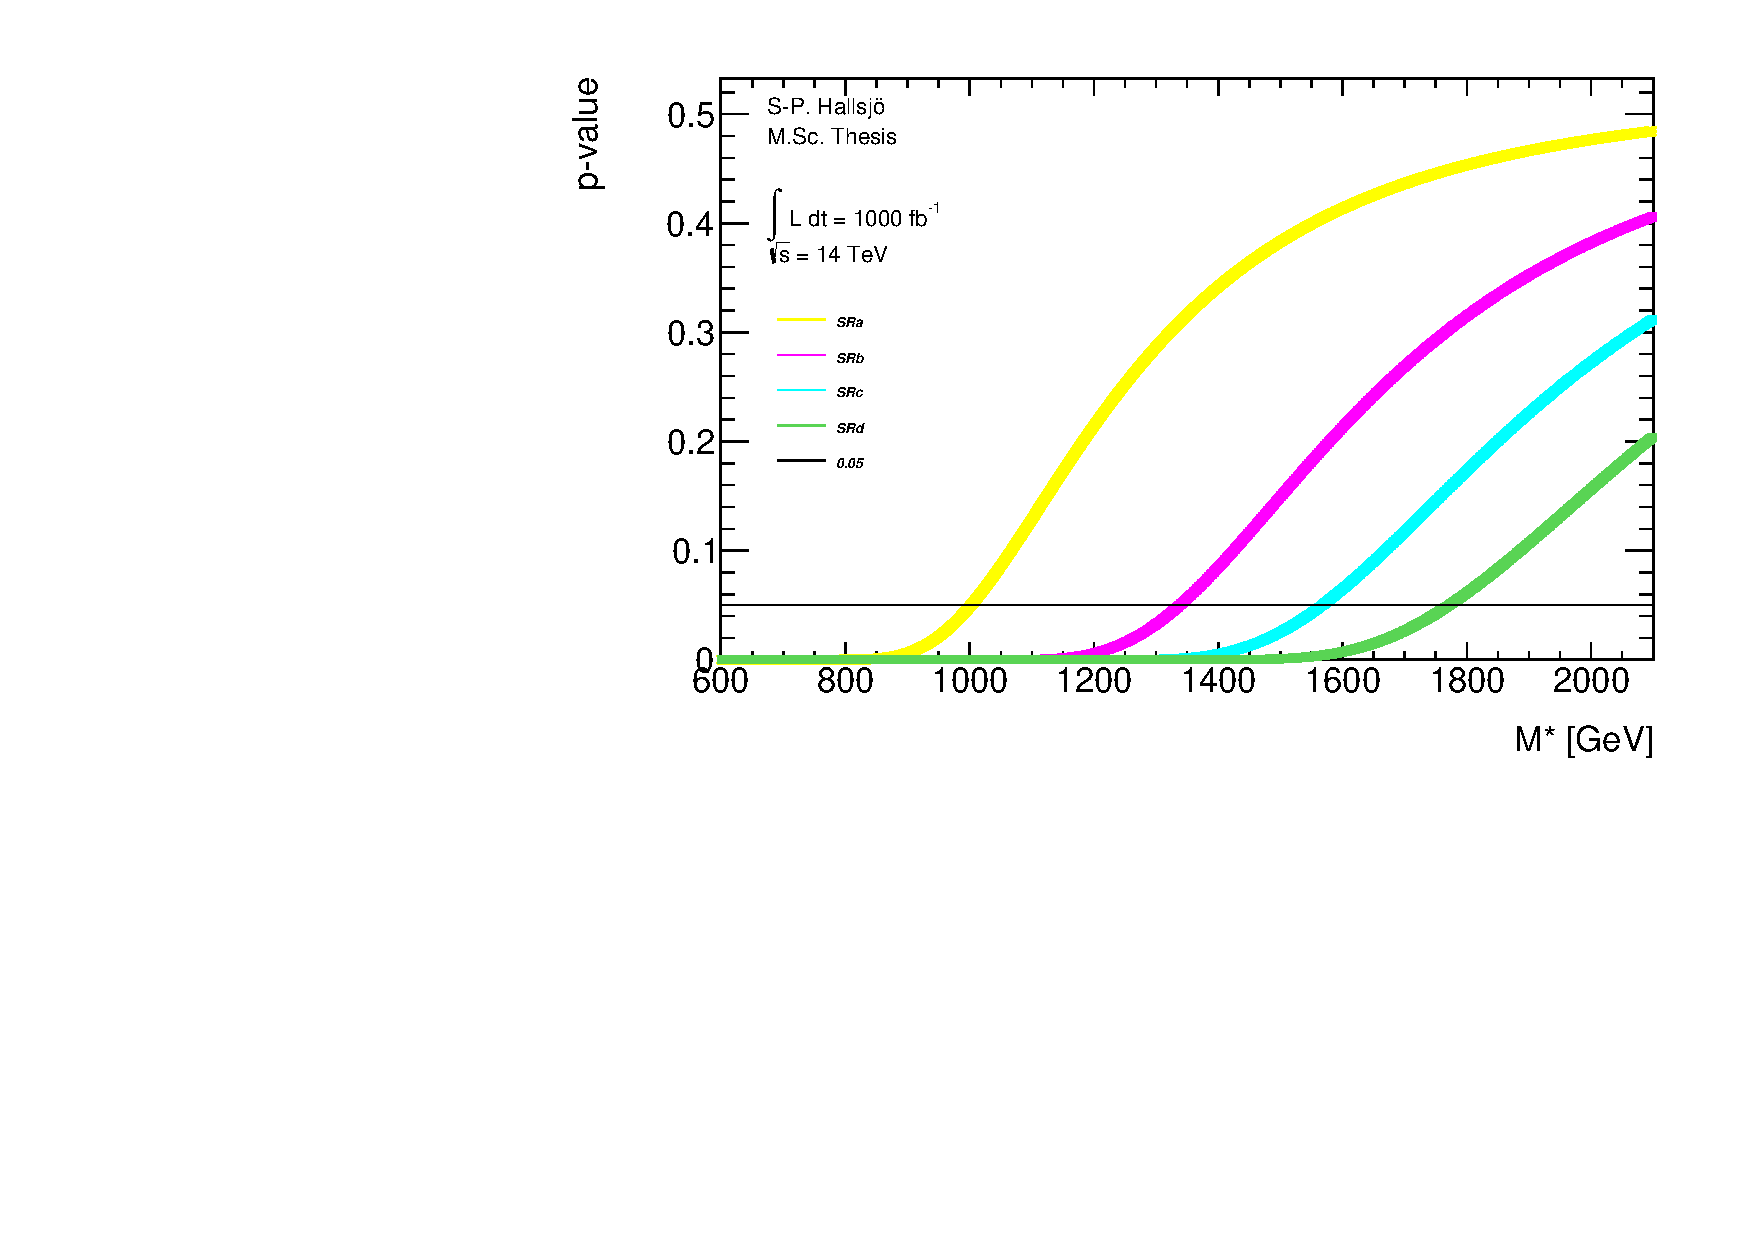
\includegraphics[width=0.5\textwidth]{pvald5008truth.pdf}
    }
    \caption{Limits of the mass suppression on a truth level for error model 0.08.}
    \label{fig:SRnewMr}
  \end{figure}

Calculating the instersection between these lines and 0.05 results in, tables~\ref{tab:masssupp002}-~\ref{tab:masssupp2010} for both a dark matter mass of 50 GeV and at 400 GeV at the different error models.

\begin{table}[ht]
\begin{center}
\begin{tabular}{|l|l|l|}
\hline
Signal region & Truth [GeV]& Reco [GeV]\\ \hline
SR1, symmetric 350 GeV &1407&1402\\
SR2, 600&1936&1934\\
SR3, 800&2227&2226\\
SR4, 1000&2404&2406\\ \hline
SRa, symmetric 350 GeV &1425&1421\\
SRb, asymmetric 600 GeV &1874&1803\\
SRc, 800&2169&2125\\
SRd, 1000&2365&2340\\ \hline
\end{tabular}
\caption{Limits on mass suppression scales in GeV given for mDm=50 GeV and the 0.02 error model.}
\label{tab:masssupp002}
\end{center}
\end{table}

\begin{table}[ht]
\begin{center}
\begin{tabular}{|l|l|l|}
\hline
Signal region & Truth [GeV]& Reco [GeV]\\ \hline
SR1&1002&999\\
SR2&1384&1382\\
SR3&1617&1619\\
SR4&1825&1834\\ \hline
SRa&1338&1286\\
SRb&1356&1303\\
SRc&1567&1533\\
SRd&1771&1745\\ \hline
\end{tabular}
\caption{Limits on mass suppression scales in GeV given for mDm=50 GeV and the 0.08 error model.}
\label{tab:masssupp010}
\end{center}
\end{table}

\begin{table}[ht!]
\begin{center}
\begin{tabular}{|l|l|l|}
\hline
Signal region & Truth [GeV]& Reco [GeV]\\ \hline
SR1, symmetric 350 Gev &1333&1329\\
SR2, 600&18481&1847\\
SR3, 800&2162&2163\\
SR4, 1000&2332&2303\\ \hline
SRa, symmetric 350 Gev&1350&1346\\
SRb, asymmetric 600 Gev&1789&1721\\
SRc, 800&2106&2059\\
SRd, 1000&2288&2258\\ \hline
\end{tabular}
\caption{Limits on mass suppression scales in GeV given for mDm=400 GeV and the 0.02 error model.}
\label{tab:masssupp2002}
\end{center}
\end{table}

\begin{table}[ht]
\begin{center}
\begin{tabular}{|l|l|l|}
\hline
Signal region & Truth [GeV]& Reco [GeV]\\ \hline
SR1&949&946\\
SR2&1321&1320\\
SR3&1570&1573\\
SR4&1770&1755\\ \hline

SRa&961&959\\
SRb&1277&1228\\
SRc&1521&1484\\
SRd&1714&1684\\ \hline
\end{tabular}
\caption{Limits on mass suppression scales in GeV given for mDm=400 GeV and the 0.08 error model.}

\label{tab:masssupp2010}
\end{center}
\end{table}

What should be noted from these tables is the significant difference between the different signals regions, especially between 4 and d which are similar apart from the lead jet momenta cut. Also how small the effect from pile-up seems to be and the increase in dark matter mass.

\newpage
\subsection{Limit on mediator mass}\label{sec:res:subsec:Mm}
For the vector mediator modes as described in \subsectionref{sec:signal:subsec:vecmed} limits on which models can be excluded have been calculated. This is done by calculating which models the p-value is $<0.05$. This is done using the two different error models as described in \subsectionref{subsec:figmer} as figures of merit. All signals which have been used can be found in \ref{livecmedpro}.


 \begin{figure}[H] %!ht
    \subfloat[A signal model given in log-scale which is not blocked by the amound of background and is thus excludable. \label{fig:sigback:1}]{%
     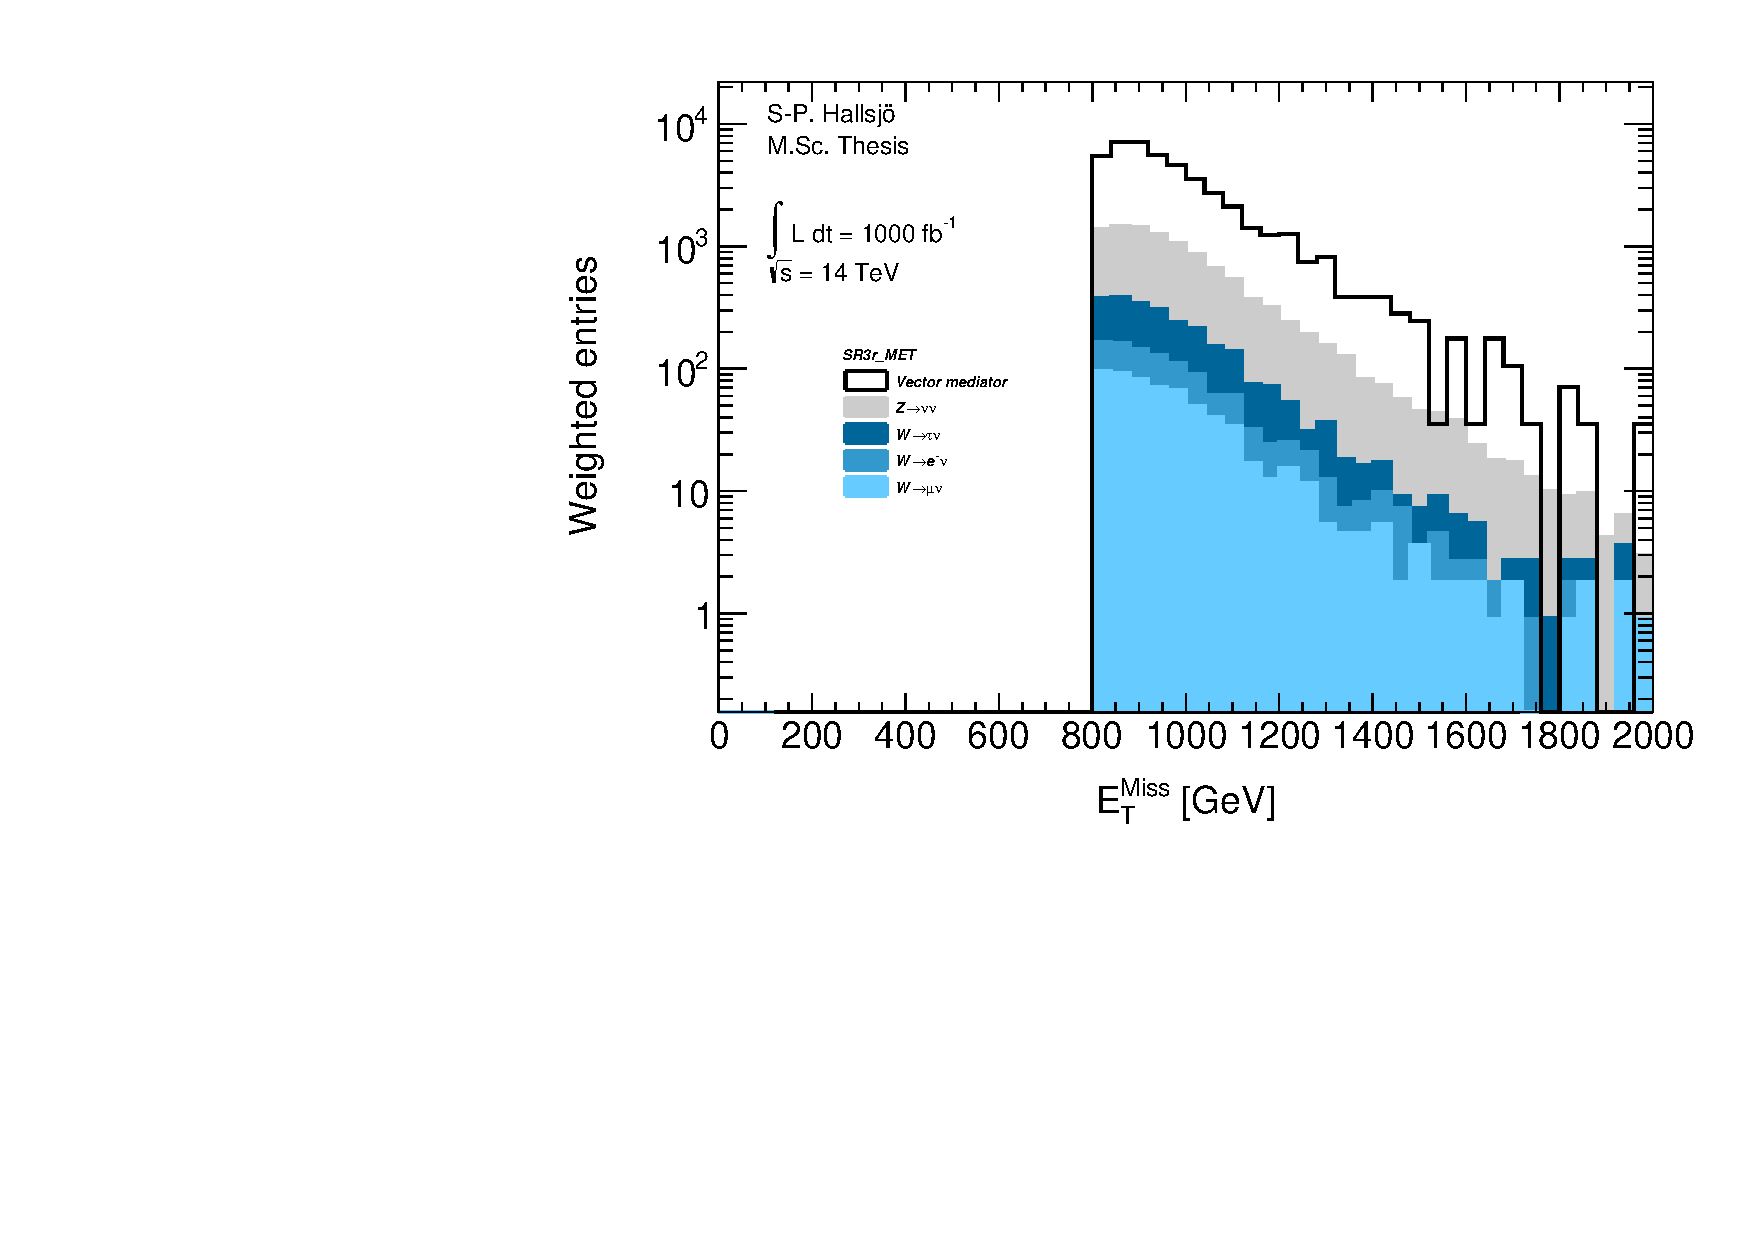
\includegraphics[width=0.5\textwidth]{mediator2.pdf}
    }
    \hfill
    \subfloat[A signal model given in log-scale which is blocked by the amound of background and is thus nonexcludable. \label{fig:sigbacktau:2}]{%
      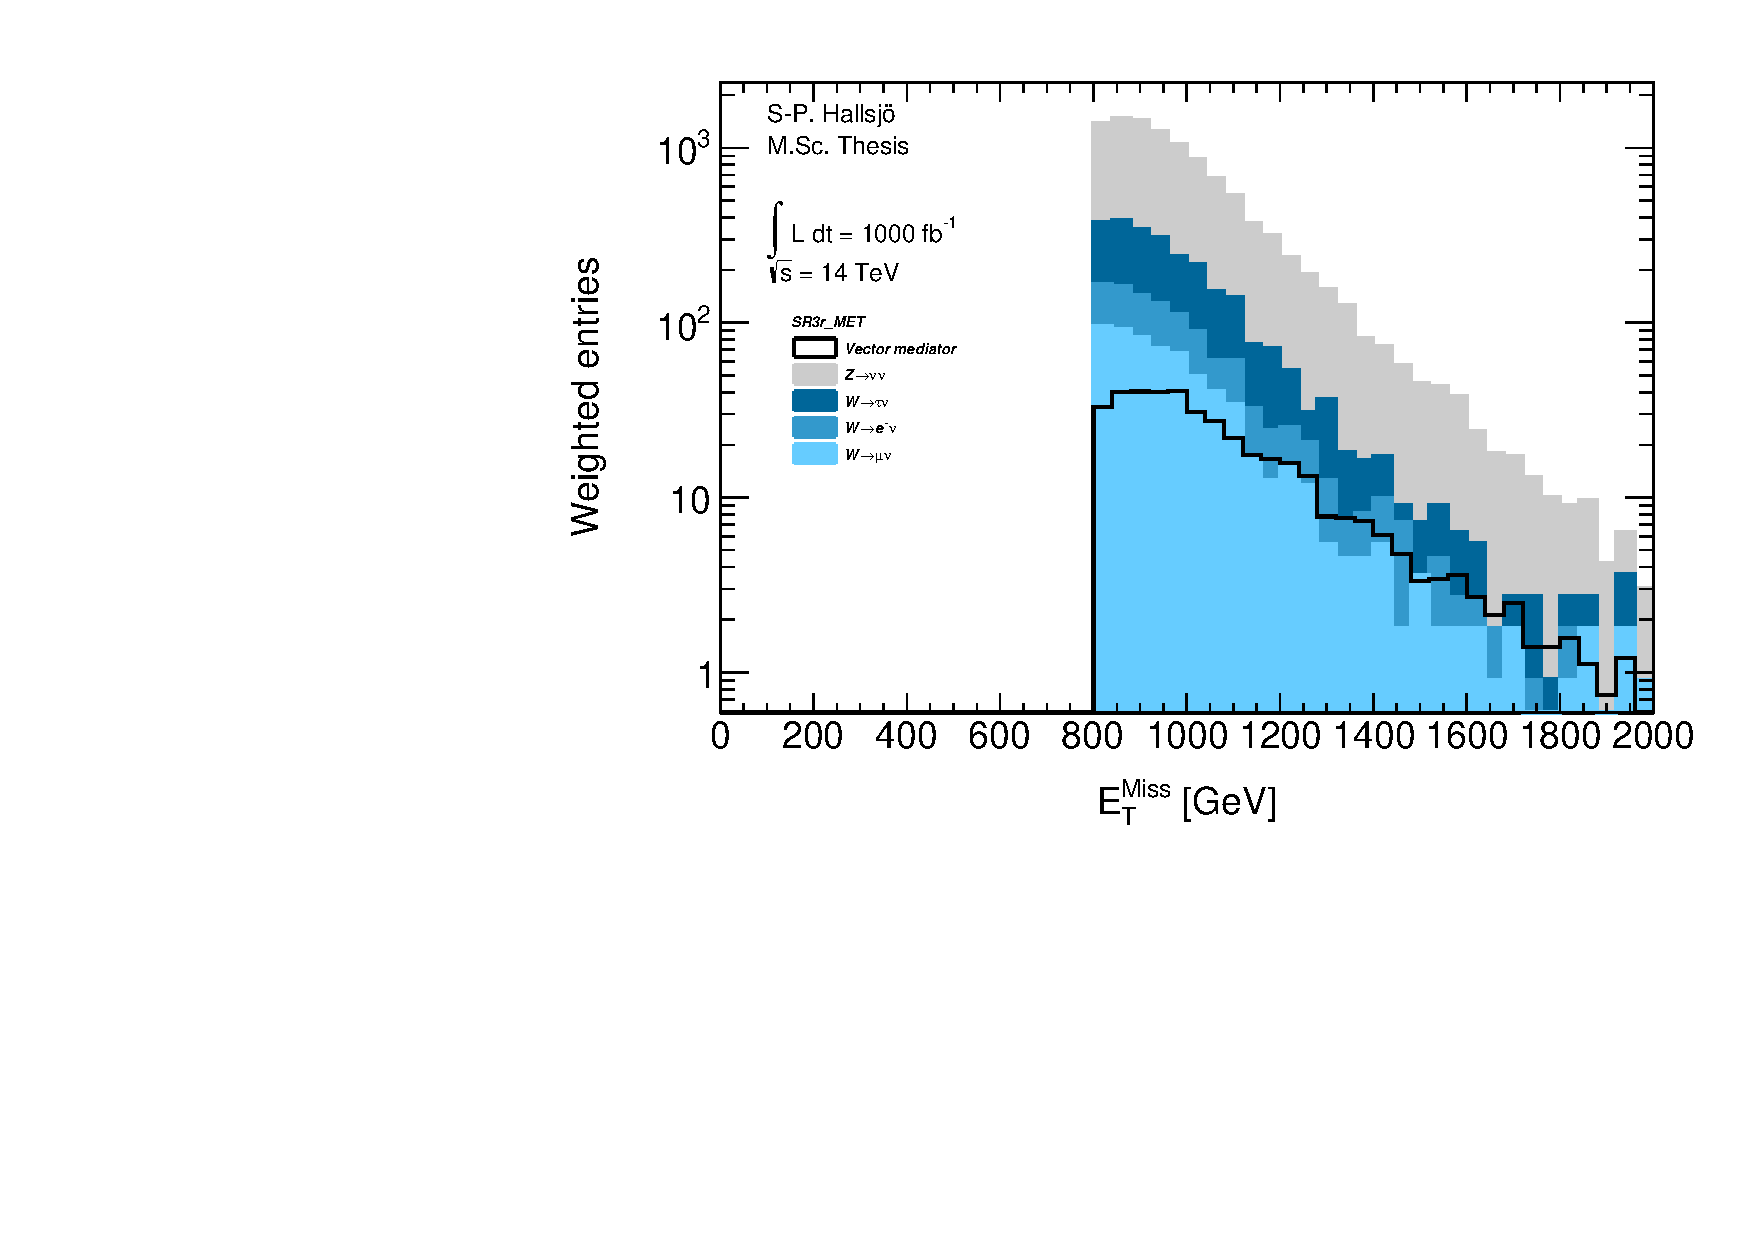
\includegraphics[width=0.5\textwidth]{mediator6.pdf}
    }
    \caption{Signal on background plot for E$^{Miss}_T$ on reco level in SR3 to illustrate a signal which is excludable and one which is not. }
    \label{fig:sigback}
  \end{figure}

To set a limit on the mediator mass the p-value is calculated in different signal regions for the different signal models with different mediator mass. As an example a plot of this in signal region d is given in \figureref{fig:modelex} where the p-value of the models is plotted against the increasing mediator mass for different widths and dark matter masses. The result of which models are excludable, thus with a p-value$<0.05$ are given in tables \ref{tab:mediatorpass} and \ref{tab:mediatorpass2}.

 \begin{figure}[H] %!ht
    \subfloat[P-values at reco level for different mediator masses and dark matter masses at a width of m/3. \label{fig:modelex:1}]{%
     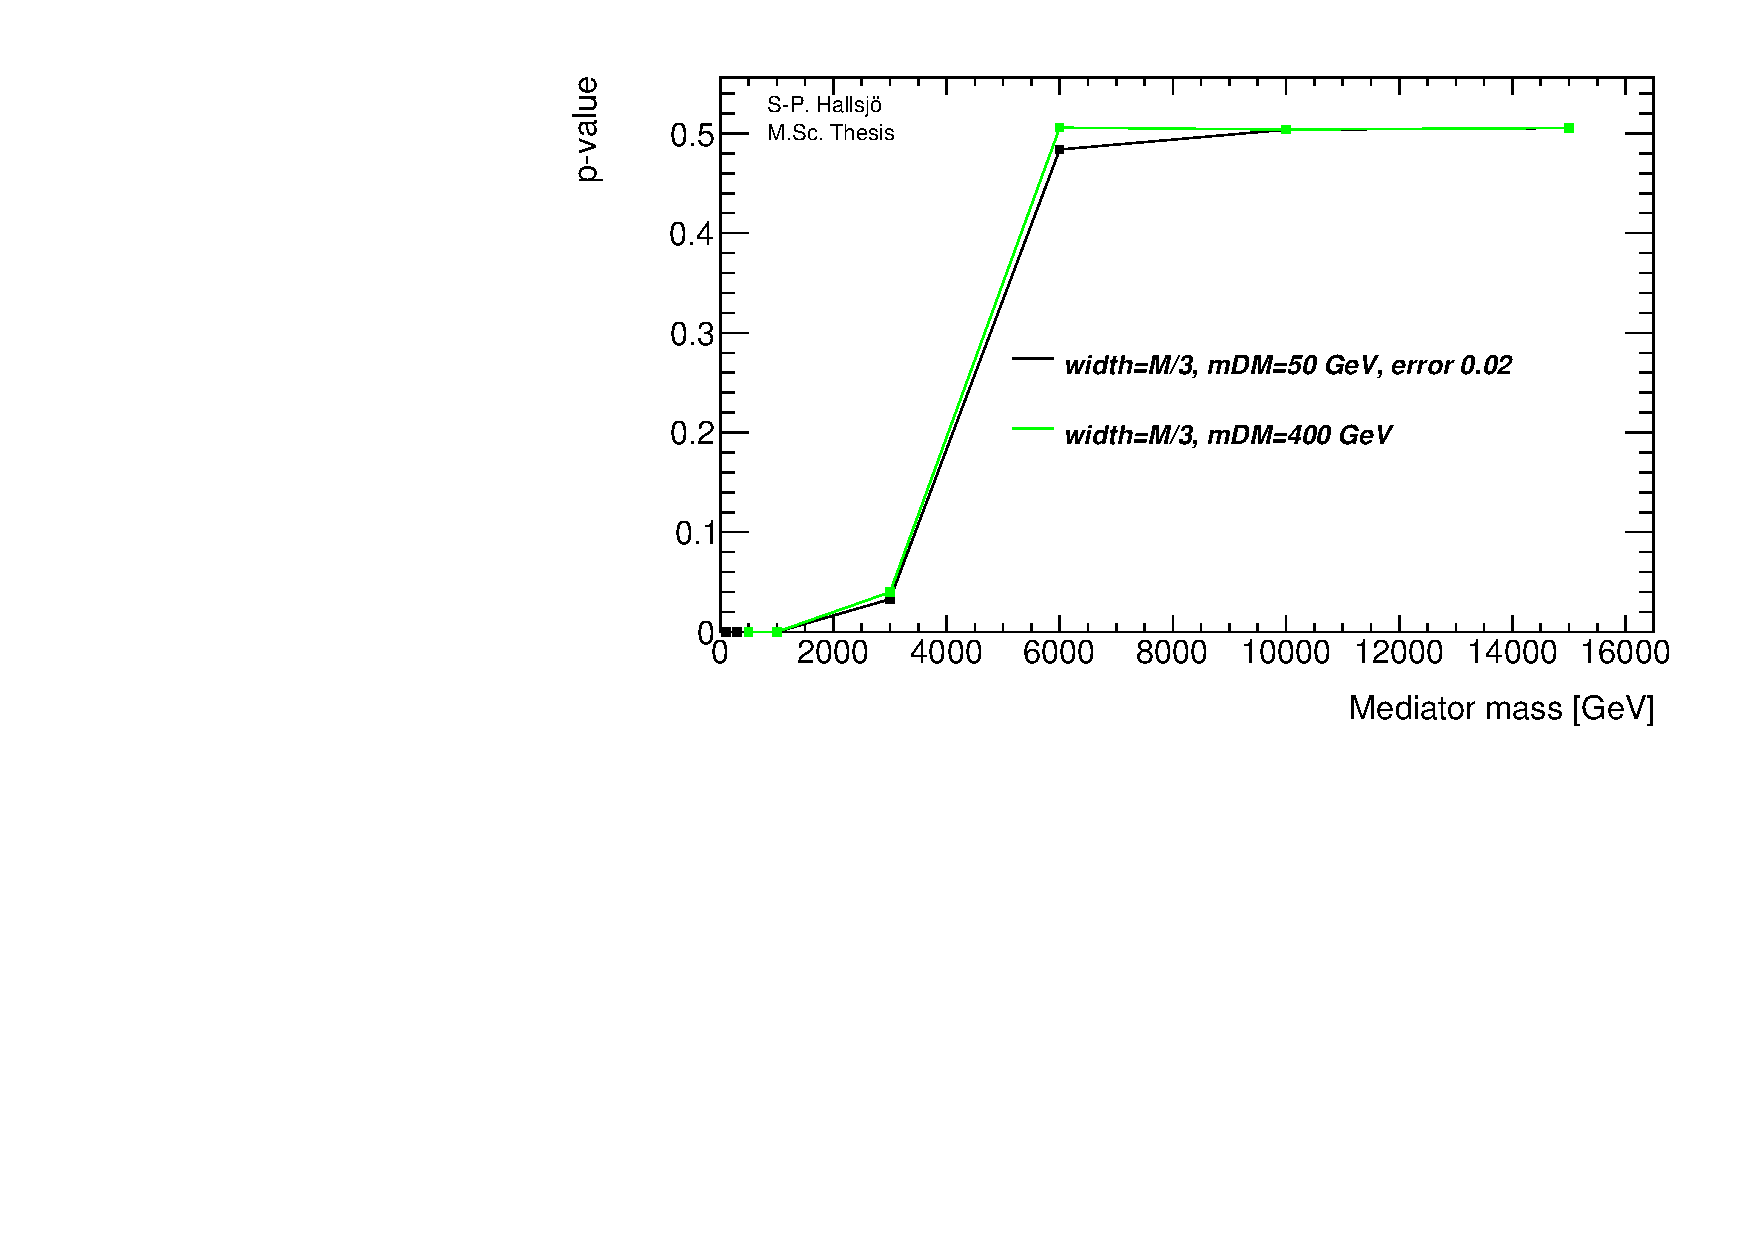
\includegraphics[width=0.5\textwidth]{reco3002.pdf}
    }
    \hfill
    \subfloat[P-values at reco level for different mediator masses and dark matter masses at a width of m/$8\pi$. \label{fig:modelex:2}]{%
      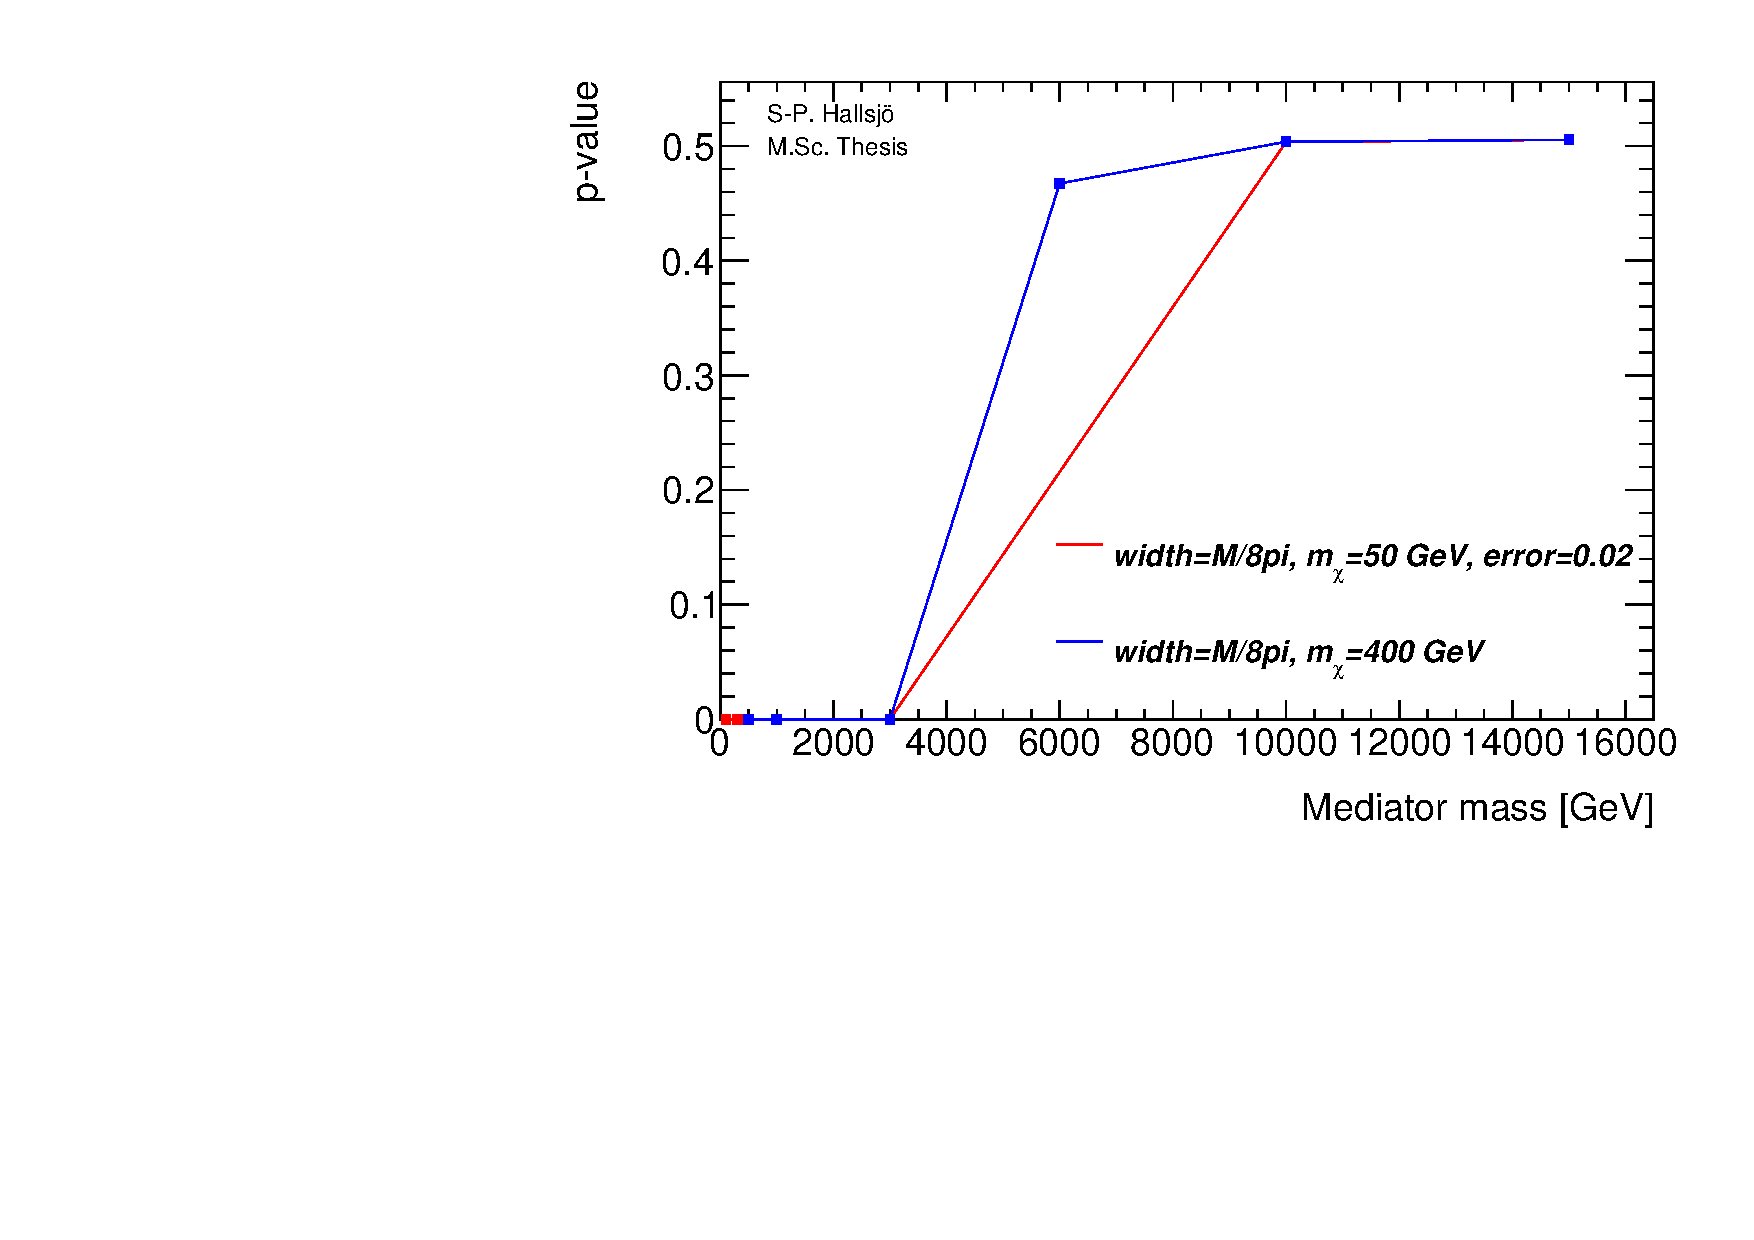
\includegraphics[width=0.5\textwidth]{reco8002.pdf}
    }
    \caption{P-values at reco level for the the different mediator masses, dark matter masses and different widths which were investigated in SRd.}
    \label{fig:modelex}
  \end{figure}



\begin{table}[ht]
\begin{center}
\begin{tabular}{|l|l|l|}
\hline
width & mDM=50 GeV & mDM=400 GeV \\ \hline
m/3 & 1000 GeV & 1000 GeV \\ \hline
m/$8\pi$ & 3000 GeV & 3000 GeV\\ \hline
\end{tabular}
\caption{Limits on which the highest mediator mass which can be excluded for different widths, different dark matter masses for truth and reco and both error models. In SR2, 3, 4, c, d.}
\label{tab:mediatorpass}
\end{center}
\end{table}
\begin{table}[ht]
\begin{center}
\begin{tabular}{|l|l|l|}
\hline
width & mDM=50 GeV & mDM=400 GeV \\ \hline
m/3 & 1000 GeV & 1000 GeV\\ \hline
m/8p & 1000 GeV & 1000 GeV\\ \hline
\end{tabular}
\caption{Limits on which the highest mediator mass which can be excluded for different widths, different dark matter masses for truth and reco and both error models. In SRb.}
\label{tab:mediatorpass2}
\end{center}
\end{table}

What can be seen in the tables is that the models are very robust when it comes to increased fluctuation in the background as indicated by the error models and with the introduction of pile-up. It is though quite interesting to see that SRb is the signal region which was worst suited for the vector mediator signals. Which by looking at the definition would suggest that the background is less susceptible to a lead jet cut than the signals.

\newpage
\section{Discussion}
\subsection{Comparison to previous results}
The background was compared to Ref. \citep{ATLAS-CONF-2012-147} altering the cross-sections of the samples used in this thesis to simulate a center of mass energy of 8 TeV instead of 14. This could unfortunately not be done for the signals as that would require new samples to be produced. As seen and some what discussed in \subsectionref{Verifying background data} the events corresponded quite nicely to the values from the paper. The discrepancies are explained by general differences between simulations and measured events, such as:
\begin{itemize}
\item The difference in W$\rightarrow\tau\nu$ can be explained by the fact that $\tau$ can not be recreated as a jet in the simulated events which it can in measured events.

\item The difference in W$\rightarrow\mu\nu$ is explained through the simulated events having a better separation of muons neutrinos and E$_T^{Miss}$.
\end{itemize}
Where the choice of a new muon veto giving more events supports the final claim.

In \tableref{Comp pval} the limits for the mass suppresion scale are given from both the paper and from this work. It is seen that the increase in luminosity and center of mass energy gives an increase of the mass supression scale by a factor of 2-3.

\begin{table}[ht]
\begin{center}
\begin{tabular}{|l|l|l|}
\hline
Dark matter mass & From simulation & From paper \\ \hline
50 GeV & 1960 GeV &800 GeV \\
400 GeV & 1871 GeV & 700 GeV \\ \hline
\end{tabular}
\caption{M* values in SR2 from both simulation at 14 TeV, 1000fb$^{-1}$ and from Ref. \citep{ATLAS-CONF-2012-147} at 8 TeV and 10fb$^{-1}$. }
\label{Comp pval}
\end{center}
\end{table}

\subsection{Effect of the high luminosity}\label{subsec:hleff}
As seen in \sectionref{chap:sig:sec:res}, the effect of a pile-up rate of 140 is minute in the signal regions chosen. The primary focus of this thesis was to look at the effect of pile-up, and try to mitigate the effect of it. However it is shown here that by choosing signal regions with a high enough requirement the effect is minute. Thus the focus was shifted to perform a more in-depth mono-jet analysis of different Dm signal models. This models were specifically the vector mediators.

For the mass suppression scale, as seen in \subsectionref{sec:res:subsec:m*}, comparing the truth values against the reco values the difference is at most $<5 \% $. Thus these signal regions are preferable for use in the high luminosity upgrade. 

Regarding the mediator models, as discussed in \subsectionref{sec:res:subsec:Mm} the models are sensitive to exclusion regardless of truth or reco. This suggests that the different models are very robust or that the effect of pile-up is negligible. However the later is more probable since a tougher error model produces the same results.

\newpage
\section{Conclusion}
\subsection{Limit on M*}
The limits can be found in \subsectionref{sec:res:subsec:m*} and are 2-3 times better than previous results at 8 TeV and 10fb$^{-1}$.

\subsection{Limit on mediator mass}
The limits can be found in \subsectionref{sec:res:subsec:Mm} and is the first result done with these models and thus can not be compared.

\subsection{Effect of the high luminosity}
At a pile-up level of 140 the effect is at most $<5\%$ for the mass suppression scale and does not affect the vector mediator models which are robust as discussed in \subsectionref{subsec:hleff}.